\documentclass[12pt]{report} % Times New Roman, 12pt
%\usepackage{gscale_thesis_singlespace} % Single spaced thesis
\usepackage{gscale_thesis_doublespace} % Double spaced thesis
\usepackage{fancyheadings} % Header and footer styling
\usepackage{natbib} % Bibliography formatting
\usepackage{setspace} % Allows double spacing but skips headers/footers
\setcounter{tocdepth}{1} % Limits the TOC to chapter and section names

% Additional packages
\usepackage{graphicx} % Allows the inclusion of figures
\usepackage{subcaption} % Allows captions to be added to subfigures
\usepackage[justification=centering]{caption} % Centres caption text
\usepackage{array} % Used for table formatting
\newcolumntype{P}[1]{>{\raggedright\let\newline\\\arraybackslash\hspace{0pt}}m{#1}}
\usepackage{booktabs} % Fancy-style tables
\usepackage{longtable} % Allows for tables that are more than one page long
\usepackage{float} % Better figure placement control
\usepackage{enumerate} % Numbered lists
\usepackage[shortlabels]{enumitem} % For controlling enumerate labels
\usepackage[shortcuts]{extdash} % Allows manual hyphenation of hypenated words
\usepackage{amsmath} % Non-standard math symbols
\usepackage{amsfonts} % Extended fonts for mathematics

\usepackage[hidelinks]{hyperref} % Linking to LaTeX labels and external URLs

\numberwithin{equation}{section} % Numbers equations based on their section
\setcounter{tocdepth}{2}
% ********************************
\begin{document}
\title{Reverse Engineering Microservices for Enhanced Insights}
\halftitle{Reverse Engineering Microservices} % 60 Characters Max. Including Spaces

\author{Muhammad Waqar Ul Hassan Awan}
\shortauthor{Waqar Awan} % Used for page header

\dept{Computing and Software}
\field{Software Engineering} % What field your thesis is in (e.g. Software Engineering)

\prevdegreeone{M.Eng. Computing and Software,\\ McMaster University, Hamilton, Canada}
\prevdegreetwo{M.Eng.} % Just your degree's field

\submitdate{March 2025} % Use the month's full spelling e.g. November
\copyrightyear{2025} % Year you are submitting this, usually your graduation 
%year

\doctype{Report} % ``Report'' or ``Thesis'' or whatever you need
\degree{Master of Engineering} % The degree you get when you submit this
\degreeabbrv{M.Eng.}
\principaladviser{Dr. Sébastien Mosser} % Your Supervisor
 % LaTeX variables for preface pages/headers
    
\beforepreface % Half title page, title page, declaration page   
  \prefacesection{Lay Abstract}

A lay abstract of not more 150 words must be included explaining the key goals and contributions of the thesis in lay terms that is accessible to the general public.  % Lay Abstract
  \prefacesection{Abstract}

Modern software systems have become significantly complex with the growing demand for features, and the need for them to be efficient and reliable has also increased. To manage this complexity, software developers have adopted advanced architectures. However, over the years, as new features are added, software systems tend to become less reliable, requiring regular maintenance. Maintaining such large systems is not a simple task, and a significant amount of resources is needed just to understand and debug even small issues. Among the various solutions to address this problem, reverse engineering appears to be one of the most feasible options, as it helps visualize and analyze the problem at hand. Surprisingly, the tools available for reverse engineering large distributed systems are limited, and those that do exist are not very flexible in terms of supporting different technologies or focusing on specific parts of an application. This report presents a framework capable of reverse engineering the static source code of any distributed system using the Unified Data Source (UDS) approach. We will consider real-world scenarios that commonly arise during software maintenance and use a microservices-based application to demonstrate the framework's effectiveness. By reverse engineering specific parts of the application, we aim to validate the practicality and credibility of our approach in real-world applications. % Abstract
  %\thispagestyle{empty}
\null\vfill
\begin{center}
%\textbf{Dedications}
%\linebreak
\textsl{Your Dedication \\ Optional second line}
\end{center}
\vfill
 % Dedication
  \prefacesection{Acknowledgements}

I want to express my sincere gratitude to my supervisor, \textbf{Dr. Sébastien Mosser}, for his support, guidance, and patience throughout my master’s studies. His knowledge and mentorship have been invaluable, and I truly appreciate the time and effort he has put into helping me complete this report. His advice and encouragement made it easier for me to complete my project.
\vspace{10pt}

A big thank you to my \textbf{family}, especially my mom and dad, for always supporting me in every way possible. Your encouragement, love, and financial support have made this journey easier, and I can’t thank you enough for always believing in me.
\vspace{10pt}

I also want to thank McMaster University for giving me the opportunity to study in such a great environment. A special thanks to all my professors for their guidance, teaching, and support throughout my master’s degree. % Acknowledgements
  \referencepages % Table of Contents, List of Figures, List of Tables
  \prefacesection{Abbreviations}

\section*{Abbreviations}
\begin{description}[font=\rmfamily\bfseries, leftmargin=3cm, style=nextline]
	\item[SST] Single source of truth
	\item[UDS] Unified data source
	\item[RE] Reverse engineering
	\item[SRE] Software reverse engineering
	\item[DSL] Domain-specific language
	\item[CI] Continuous Integration
	\item[CD] Continuous Deployment
	\item[VCS] Version Control system
	\item[JSON] JavaScript Object Notation
\end{description}
  \academicstatement{academicachievementdeclaration}
\afterpreface
  
  \chapter{Introduction}

Developing a large software system is a complex and crucial process that requires careful planning and execution. When a stable product is built using a monolithic architecture, where a single codebase handles all business logic, years of development—adding new features and data—can make it highly prone to errors and less resilient. To address this issue, the industry adopted the \textit{``Divide and Conquer''} principle and migrated their products to microservices architecture, where each service represents a separate business logic. However, a major drawback of microservices is the difficulty of maintaining them due to multiple interconnected parts. For example, Monzo, a UK-based digital bank, has implemented a system comprising approximately 2,800 microservices and counting~\citep{monzoMicroservices}.

Some companies, including Amazon's Prime Video team, have reverted from microservices to monolithic architectures due to challenges in maintaining microservices. As a result, they reduced infrastructure costs by 90\% and improved scalability~\citep{anderson2023microservices}. Maintaining such large systems is just as crucial as building them. One effective approach to understand the internal structure of a system to make it easier to maintain is \textbf{reverse engineering}. Reverse engineering helps visualize complex and legacy systems by leveraging automatic visualization techniques to manage large systems effectively. It also aids maintainers in analyzing source code at different levels of abstraction~\citep{SVInSoftwareMaintenanceRainer}.

There are no one-size-fits-all tools available in the market that adopt the reverse engineering approach for software maintenance. For example, \textit{Rigi}\footnote{\url{https://rigi.uvic.ca/Pages/download.html}} is a tool for software reverse engineering that visualizes legacy systems. However, Rigi has limited language support, as its built-in parsers primarily support C and COBOL. Users have also reported performance issues when analyzing large systems, particularly with graphs exceeding 500 nodes~\citep{Koschke2002}. Active development of Rigi ceased in 1999, with the last official release in 2003. 

We can present a framework that can reverse engineer large distributed systems by performing static analysis on the source code and extracting useful artifacts. This process can be integrated into the CI/CD pipeline to extract real-time information with each release and present it using a visualizer. 

The primary objective of this report is to demonstrate such a framework that extracts artifacts from source code and uses the \textit{unified data source (UDS)} approach to maintain up-to-date and credible data. The extracted information is stored as nodes and edges in a graphical database, which is then connected to a visualizer for further analysis and insights based on specific requirements.

This report will answer the following questions:
\begin{enumerate}
    \item Which key components must be integrated to effectively reverse engineer any microservice architecture based system?
    \item How can data collected by probes be centralized into a unified, consistent, and real-time source to enhance accuracy and reliability?
    \item How can stored data from the source code be transformed into visually intuitive and insightful graphical representations?
\end{enumerate}

Chapter 2 provides background information and key points essential for understanding the overall concept of this project. Chapter 3 discusses the envisioning of the framework and its three key components, which address Question 1. Chapter 4 covers the implementation of probes and their integration with the unified data source, answering Question 2. Chapter 5 validates the scenarios discussed in Chapter 3 by generating graphical information and insights using the data stored in the UDS, addressing Question 3. Lastly, Chapter 6 concludes this report and explores future work that could enhance the framework's usability and practical applications.
                  
        \setcounter{figure}{0}
        \setcounter{equation}{0}
        \setcounter{table}{0}

  \chapter{Background}

This chapter provides the background information necessary to understand this report. It covers topics such as the development of large software systems, types of software systems, their maintenance, analysis, and other related concepts.

\section{The Software Lifecycle: From Idea to Execution}

Developing a large software system is a complex and crucial process that requires careful planning and execution. A large scale software system involves many interconnected components, all of which must adhere to essential software development principles. The goal is not just to write code but to build a system that is reliable, maintainable, scalable, and efficient. Ensuring the system is free of bugs and capable of adapting to future needs is as important as the initial development itself. By following these key paradigms, developers can create software that meets high standards of quality and performance.

\begin{figure}[H]
    \centering
    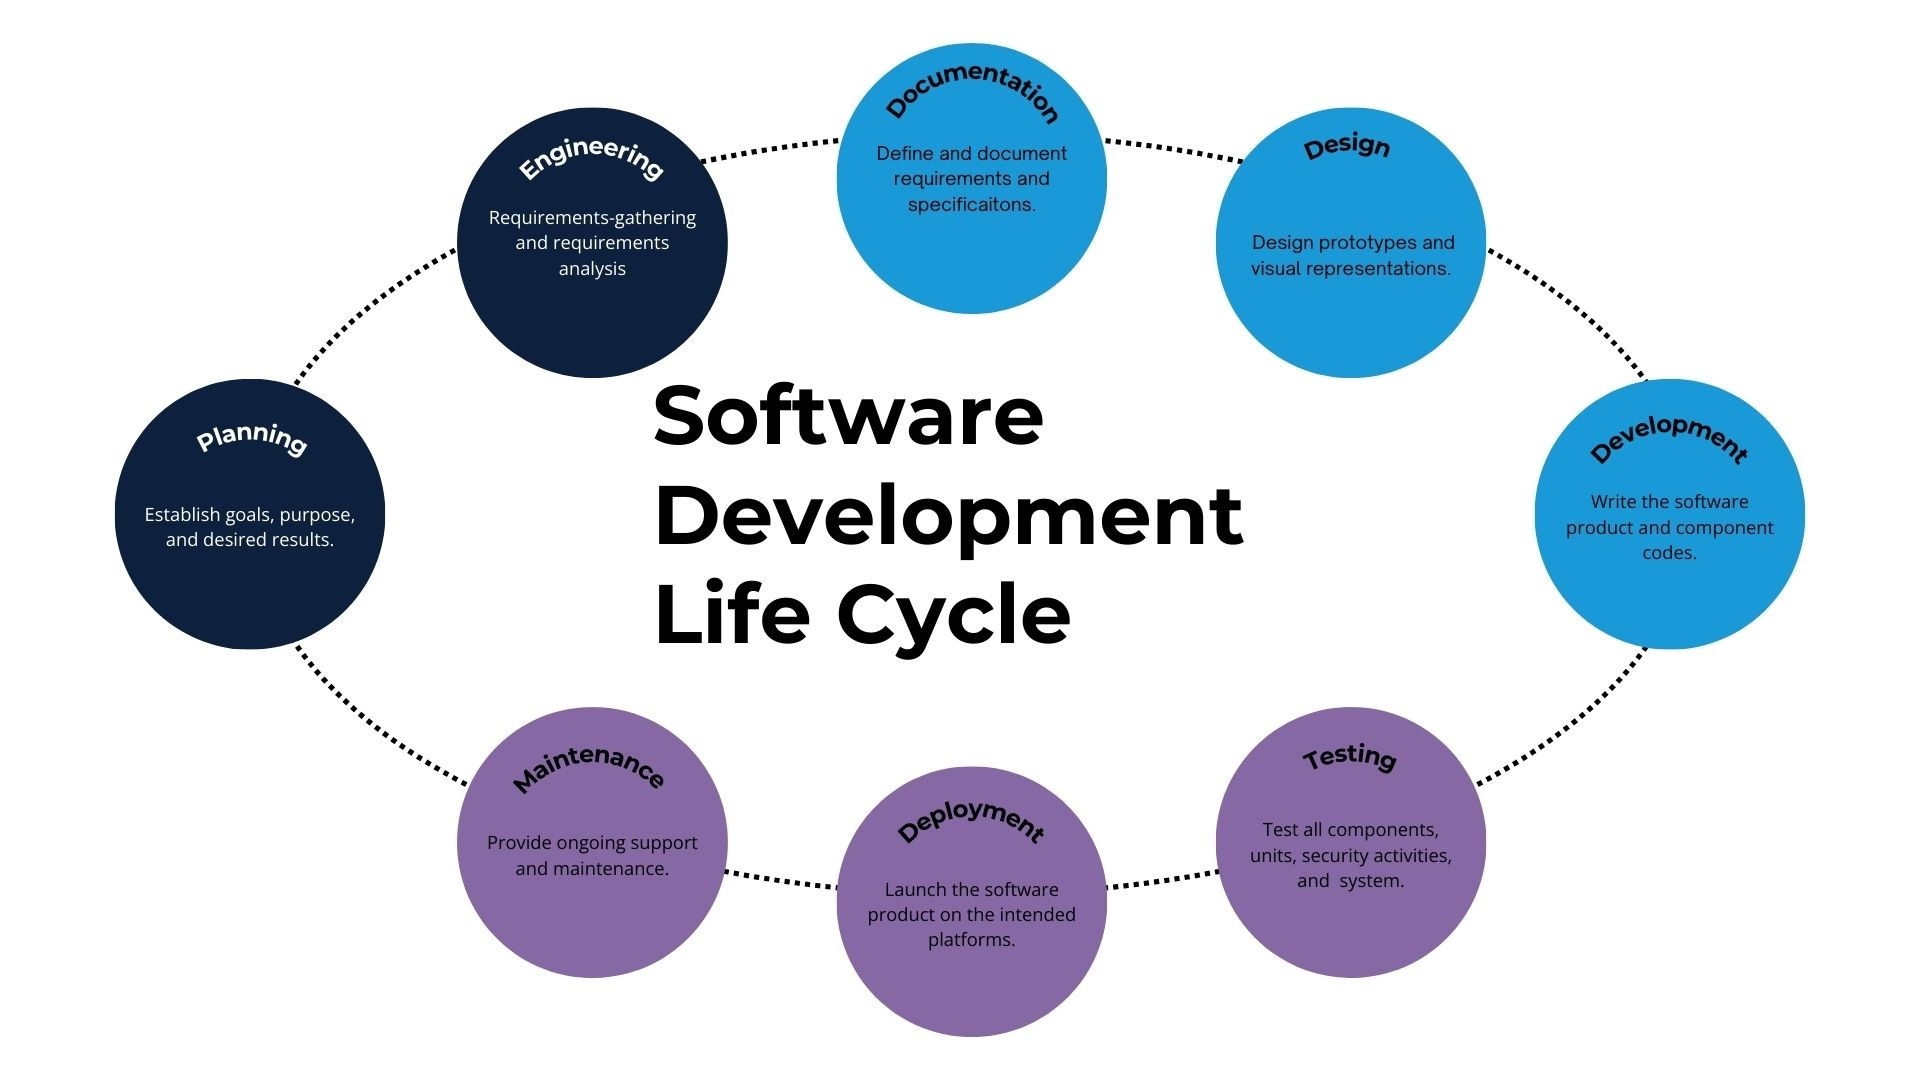
\includegraphics[width=1\textwidth]{figures/software_development.png}
    \caption{Software Development Life cycle (adapted from~\citep{sire_sdlc_2024})}
	\label{fig_background_sd}
\end{figure}

Each phase of the software development process adds an important contribution to the overall project. For example, in the planning and engineering phase, the team works closely with stakeholders to determine the functional and non-functional requirements of the project. This collaboration ensures that everyone involved understands the project's goals and technical needs. In the documentation phase, all the information gathered during planning and engineering is carefully recorded. This creates a detailed reference for the team, helping maintain consistency and clarity as the project progresses.

Following the Software Development Life Cycle (SDLC) provides several key benefits. It helps in identifying clear goals, ensures all stakeholders are on the same page, and allows for thorough testing at every stage. This structured approach produces high-quality software systems and maintains a smooth and understandable development flow. By sticking to the SDLC, teams can reduce risks, avoid confusion, and create software that meets user expectations.

Once the major development work is complete, the focus shifts towards software maintenance. Maintaining a large project becomes a significant task in itself. Updates, bug fixes, and adapting to new requirements or technologies are ongoing responsibilities. Without proper maintenance, even the best-designed systems can become outdated or difficult to use.

\section{Software Maintenance in Large Systems}

Since an already built large software system is quite complex, understanding this system requires certain strategies and tools. When a problem arises in complex software architectures, such as microservices or service-oriented architectures, resolving it often demands significant resources. These architectures consist of numerous interconnected components, and identifying the root cause of an issue can be challenging. The process may involve extensive debugging, analyzing logs, coordinating between multiple teams, and sometimes even re-evaluating design decisions. This can result in considerable time, effort, and cost being spent to restore functionality and ensure the system operates smoothly.~\citep{Folmer2005} discusses the usability issues in software systems post-development and highlights that they require significant architectural changes. In order to deal with such architectural changes, an understanding of the whole system is required, and if the system is large enough, major resources are spent fixing even minor issues.

~\citep{SeMaintainance2001} states that several surveys indicate that software maintenance consumes 60\% to 80\% of the total life cycle costs. Also, the maintenance costs are largely due to enhancement (often 75{-}80\%), rather than corrections. To address these challenges, there is a growing need for tools that can assist in resolving bugs and reducing maintenance overhead. Such tools should be capable of reverse engineering software systems to provide a clear and comprehensive view of the architecture. By highlighting the key components and their interactions, these tools make it easier for developers to understand the system, identify issues, and perform necessary tasks efficiently. This not only simplifies debugging but also enhances the overall maintainability of the software, ensuring smoother operation and reduced downtime.

\begin{figure}[H]
    \centering
    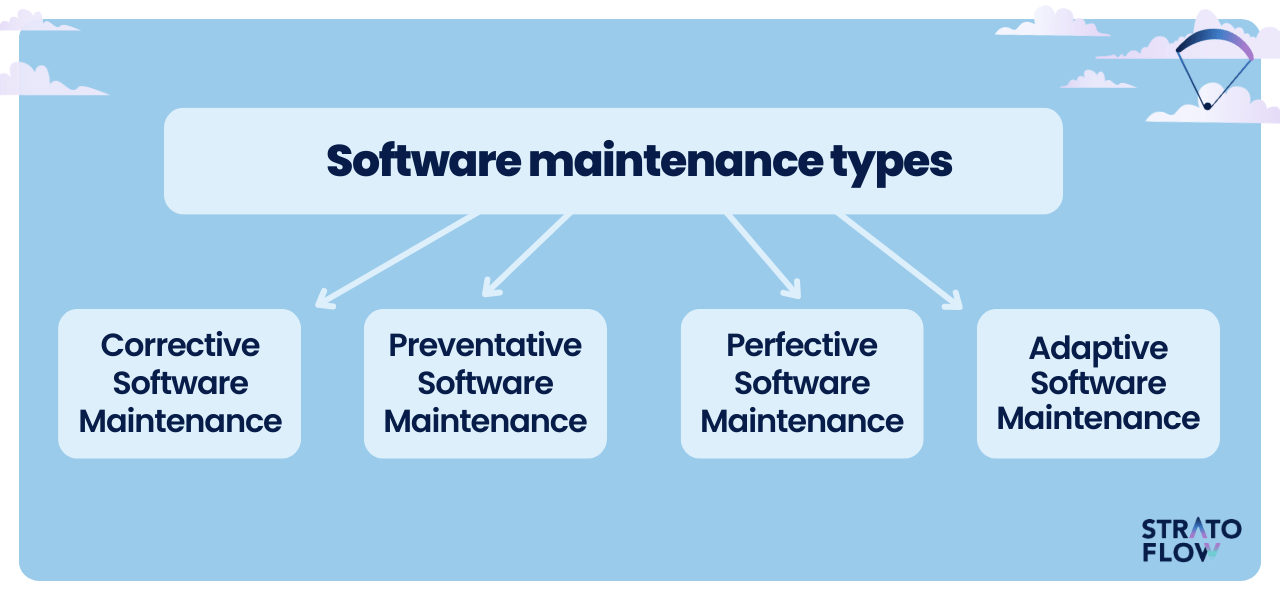
\includegraphics[width=0.9\textwidth]{figures/se_maintenance.png}
    \caption[Software Maintenance Types]{Software Maintenance Types (adapted from~\cite{stratoflow2025})}
	\label{fig_se_maintenance}
\end{figure}

\section{Software Architectures}
Software architecture is the fundamental structure of a software system.~\citep{sei_software_architecture} refers software architectures as the ``representation of the design decisions related to overall system structure and behavior. Architecture helps stakeholders understand and analyze how the system will achieve essential qualities such as modifiability, availability, and security''.

Each architecture has its own pros and cons. There are different types of software architectures adopted or sometimes introduced in order to solve certain issues. The most important ones that are necessary to be understood for this report are monolithic and microservices architectures.

\subsection{Monolithic Architecture}
Monolithic architecture is a traditional software development design paradigm where an application is built as a single, unified unit. All the components of the system are tightly coupled and dependent on each other. The monolithic architecture is simple, easier to design, develop and test and usually have easier deployment process as compared to some other architectures.

\subsection{Microservice Architecture}
Microservice architecture is a software design in which a system is built as a collection of small, independent, and loosely coupled services. Each service is designed to keep in mind the Single-responsibility principle and hence have a specific function, operates independently and communicates with other services typically using HTTP or messaging queues. Microservice architecture is easier to scale, flexible, autonomous and more resilient than other architectures, especially monolithic. 

\begin{figure}[H]
    \centering
    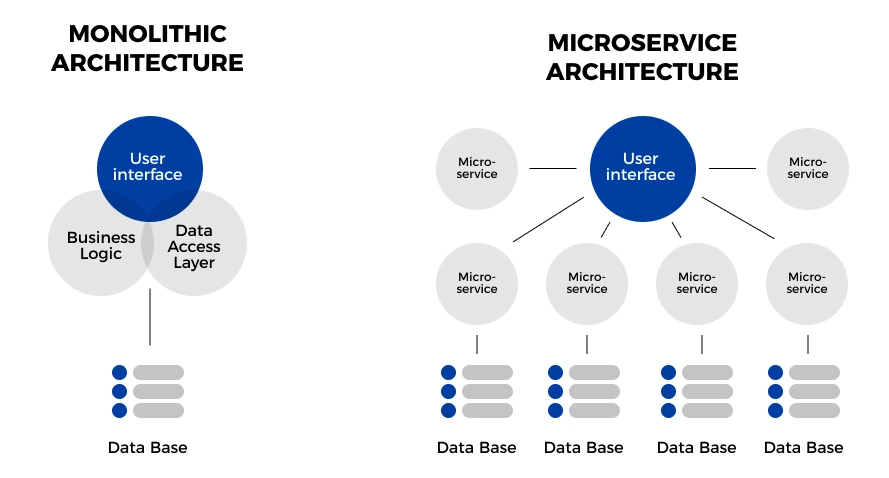
\includegraphics[width=0.9\textwidth]{figures/monolithic_microservices.png}
    \caption{Monolithic vs Microservices Architecture (adapted from~\cite{atlassian_microservices_vs_monolith})}
	\label{fig_background_monolithic_microservices}
\end{figure}

The figure~\ref{fig_background_monolithic_microservices} shows the difference between the monolithic and microservice architecture. In monolithic, all the components of the software system are combined in a single unit whereas in microservice architecture, the whole system is divided into smaller autonomous components. These individual components are easier to manage, scale, maintain and debug.

One of the key challenges in software development is understanding the system’s architecture after the major development process is completed or stabilized. Developing a software system often takes years of effort and significant resources. As a result, fully grasping its complexity can be difficult, especially for teams that were not involved in the original development.

To overcome this challenge, proper documentation, well-defined workflows, and effective knowledge transfer are essential. However, even with these measures, there are instances where critical system insights are required to diagnose issues efficiently. In such cases, improved documentation and deeper system analysis become necessary. This is why \textbf{reverse engineering} is often applied to existing or legacy systems to gain a clear understanding of their structure and functionality.

\section{Understanding Reverse Engineering}  
\citep{digitalai_reverse_engineering} states that 
\begin{tcolorbox}[colback=gray!10, colframe=gray!20]
	``The goal of reverse engineering is to reveal the logic, features, and functionalities embedded within the software.''
\end{tcolorbox}

An article by~\citep{twoFacesOfSRE} discusses that software reverse engineering can be achieved through several approaches:
\begin{itemize}
    \item \textbf{Observation-Based Analysis:} Involves studying the exchange of information within the software to infer its functionality and behavior.
    \item \textbf{Disassembly:} Utilizes a disassembler to interpret and analyze the program's raw machine code.
    \item \textbf{Decompilation:} Employs a decompiler to attempt reconstruction of the program’s source code in a high-level language, starting from machine code or bytecode.
\end{itemize}

\begin{figure}[H]
    \centering
    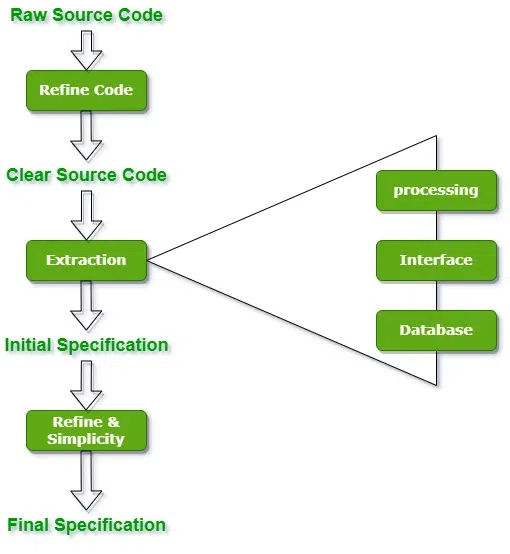
\includegraphics[width=0.75\textwidth]{figures/Reverse-Engineering.png}
    \caption{Reverse Engineering (adapted from~\cite{geeksforgeeks2024})}
	\label{fig_background_reverse_engineering}
\end{figure}

As shown in figure~\ref{fig_background_reverse_engineering}, source code is refined and analyzed to derive a final specification.

\begin{itemize}
    \item The process begins with the raw source code of a software application.
    \item The raw source code is refined to make it cleaner, more organized, and readable by removing unnecessary parts.
    \item The process of extraction identifies key elements of the system.
    \item An initial specification of the system is created, outlining the system's structure and behavior.
    \item The initial specification is then further refined to ensure simplicity and reducing complexity.
    \item The process concludes with a final specification, which is a clear description of the system's design, functionality, and architecture.
\end{itemize}


In the later chapters of this report, we will discuss a framework that uses static analysis of source code. This framework aids in reverse engineering by disassembling the system and generating valuable insights.
                  
        \setcounter{figure}{0}
        \setcounter{equation}{0}
        \setcounter{table}{0}
        
  \chapter{Vision and Technical Strategy}

The development of a large software system is a very critical process and there are a lot of parts that are involved in a project that needs to follow key software development paradigms so that it is easy to maintain. Its not just about writing code, its about creating a system that is bug free, easy to maintain, scalable and efficient.

Since an already built large software system is quite complex, so understanding this system requires certain strategies and tools.~\citep{Folmer2005} discusses about the useability issues in the software systems post-development and they require significant architectural changes. In order to deal with such architectural changes, understanding of the whole system is required and if the system is large enough, major resources are spent to fix even minor issues. 

~\citep{SeMaintainance2001} states that several surveys indicate that software maintenance consumes 60\% to 80\% of the total life cycle costs. Also the maintenance costs are largely due to enhancement (often 75{-}80\%), rather than corrections. So a framework should be developed that could solve these issues by doing reverse engineering on the software systems and showing the importants aspects of the software architecture in order to make it easy to understand and perform the required tasks.

\begin{figure}[ht]
    \centering
    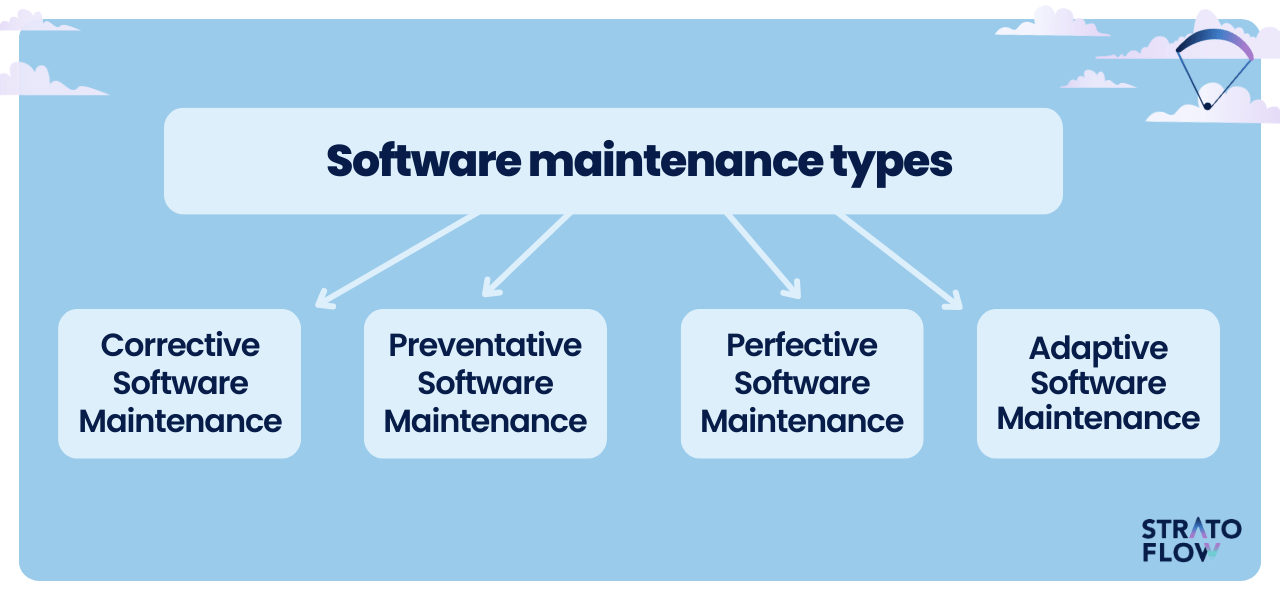
\includegraphics[width=0.8\textwidth]{figures/se_maintenance.png}
    \caption[Software Maintenance Types]{Software Maintenance Types (adapted from~\cite{stratoflow2025})}
	\label{fig_se_maintenance}
\end{figure}

\section{Vision}\label{sec:vision}

Keeping in mind the above discussed issues, there is a need for an approach in which the software system could be analyzed, undergo processing and produce useful informations that can be used to provide enhanced insights about the project. The vision is to use a framework consisting of 3 components: 
\nameref{subsec:component-probes}, \nameref{subsec:component-sst} and \nameref{subsec:component-visualizer}. All three components will be discussed in detail in section{ }\ref{sec:tech-strategy}.

In this report, we will discuss,implement and validate this framework by extrac
ting static information from a project. In the future, this can be implemented/integrated with the CI/CD pipeline and provide dynamic information from the projects. The test project used in this report is Java spring framework based project called petclinic. Read more about this project from \href{https://github.com/spring-petclinic/spring-petclinic-microservices}
{spring petclinic microservices github repository}~\citep{spring-petclinic}.

Moreover, our approach will be mainly focused on the unified data source (UDS) approach.~\citep{unifiedData2025} states that Unified Data refers to the integration and consolidation of data from various sources into a single, cohesive framework. This approach allows organizations to streamline their data management processes, ensuring that all data is accessible and usable across different departments and applications. By unifying data, businesses can eliminate silos, reduce redundancy, and enhance the overall quality of their data analytics efforts. It means that consistent, up-to-date and valid data will be available using the UDS technique.


\section{Technical Strategy}\label{sec:tech-strategy}

This section provides a detailed discussion of the components in the framework. It also includes an analysis of the probes used to prove the framework's credibility, their use cases, and their benefits. After that, it discusses the unified data source (UDS) and, finally, the visualizer component.

\subsection{Framework Components}\label{subsec:framework-components}

The framework contains three main components.
\begin{itemize}
    \item \nameref{subsec:component-probes}
    \item \nameref{subsec:component-sst}
    \item \nameref{subsec:component-visualizer}
\end{itemize}


\subsection{Probes}\label{subsec:component-probes}

The first component of the framework consists of \textbf{probes}. Probes represent distinct informational artifacts that are systematically extracted from software systems to provide insights and actionable data. In the context of this report, we have several use cases and extracted specific pieces of information that are detailed in the below subsections. These probes serve as the foundational elements for gathering critical data points that enable analysis and decision-making. 

Looking forward, this concept can be expanded to more complex and targeted informational needs. By refining the scope and nature of the probes, we can tailor the probes according to our needs and to capture more refined data, addressing evolving requirements and insights that drive meaningful outcomes. This flexibility ensures that as the systems grow or change, the framework remains relevant and capable of producing deeper, more impactful information.

Given below are some of the probes that are implemented as part of this report in order to show the credibility of the presented framework. In later chapters, their implementation will be discussed at length followed by the validation of each scenario discussed here.

\begin{enumerate}[leftmargin=*, label=\arabic*.]

    \item \subsubsection*{Authors Contributions}
    Author contribution probe extracts information about the developer who made the most recent changes to a method, list of all the developers who contributed to a method and highlights the developer with most contributions to a particular method. There are multiple use cases for this type of data.
	\subsubsection{Use Cases}
	\begin{itemize}[label=$\bullet$]
		\item \textbf{Bug Fix}: When a bug is found in a method, the most recent author who updated the method would have the context of the recent changes that they have made and can help diagnose and resolve the issue faster. This will help the organization increase their productivity.
		\item \textbf{Reviews}: Looking at the most recent developer would give an idea of who to reach for documentation, clarification and review of the changes.
		\item \textbf{History Tracking}: Provides insights into who and why the person made the recent changes which can be used for documentation purposes.
		\item \textbf{Identify Developers Group}: Helps identify the group of developers who worked on a particular method, which in turn enables them to share and transfer knowledge in case the top contributor of the method is unavailable.
		\item \textbf{Ownership}: Tracks if the code has been worked on collaboratively or primarily by one individual.
		\item \textbf{Refactoring}: Ensures that all the contributors can be consulted and their insights are taken before performing any major refactoring.
		\item \textbf{Knowledge and Accountability}: Identifies the subject matter expert for particular methods and assigns ownership of the method to the top contributor for accountability and guidance.
		\item \textbf{Planning}: Helps management decide who should be involved in any major changes to the method based on past contributions.
	\end{itemize}
	\subsubsection{Benefits}
	\begin{itemize}[label=$\bullet$]
		\item \textbf{Improve Communication}: Facilitates and improve communication between team members by identifying relevant stakeholders.
		\item \textbf{Enhanced Planning}: Improves resource allocation, project planning and decision making for development tasks.
		\item \textbf{Transparency}: Promotes accountability among team members by making contribution history transparent.
		\item \textbf{Efficiency}: Increases team efficiency and issue resolving by involving right people for the job.
	\end{itemize}
	
    \item \subsubsection*{File Authors}
	This probe extracts information regarding the authors of a particular file. In software development, especially in large-scale microservices architecture, understanding the list of contributors to individual files provides significant value.
	\subsubsection{Use Cases}
	\begin{itemize}[label=$\bullet$]
		\item \textbf{Ownership}: Identifying contributors of a particular file highlights the ownership and familiarity with the functionality of the file of the people associated with it.
		\item \textbf{Collaboration}: Identifying contributors reveals whether a file has been developed collaboratively or by a single individual.
		\item \textbf{Auditing and Compliance}: Contributor information is crucial for tracking accountability and compliance. Specially in open-source projects.
		\item \textbf{Maintenance}: Files with multiple contributors might lead to maintenance challenges. Having list of contributors help assign the tasks to the correct people.
		\item \textbf{Bug and Issue Assignment}: Assigning issues to contributors who are familiar with the relevant files improves resolution speed.
	\end{itemize}
	\subsubsection{Benefits}
	\begin{itemize}[label=$\bullet$]
		\item \textbf{Accountability and Quality}: Knowing who contributed to a file ensures accountability and encourages higher-quality contributions.
		\item \textbf{Team Collaboration}: Make team collaboration easier by identifying relevant stakeholders for discussions.
		\item \textbf{Reduces Risk}: Identifies files relying on single contributor which can help in workload distribution.
	\end{itemize} 

	\item \subsubsection*{Author Relation}
	This probe extracts information regarding the strength of collaboration between two authors. Greater the collaboration, great will be the strength of bond between them. The ``relation strength'' metric quantifies the level of collaboration between pairs of authors based on shared contribution to files. In collaborative software development, especially in microservices architectures, understanding the strength of relation among authors can provide valuable insights into teamwork, communication and collaboration in the development process.
	\subsubsection{Use Cases}
	\begin{itemize}[label=$\bullet$]
		\item \textbf{Collaboration Analysis}: Provides a quantitative measure of collaboration between two developers in a development team. Higher strength shows frequent joint contributions.
		\item \textbf{Planning and Resource Allocation}: Helps plan tasks and form teams for future projects by using existing strong collaboration bonds.
		\item \textbf{Knowledge Transfer}: New developers can use relation strength data to identify key collaborators within the team.
		\item \textbf{Shared Ownership}: Helps determine the shared ownership of the files, making it easier to assign maintenance tasks.
		\item \textbf{Technical Debt}: Low pairwise strengths and high number of collaborators of a file represents cohesive ownership, leading to technical debt.
	\end{itemize}
	\subsubsection{Benefits}
	\begin{itemize}[label=$\bullet$]
		\item \textbf{Improved team dynamics}: Improve team dynamics and encourages better interaction in areas with weaker team collaboration.
		\item \textbf{Fast Problem Solving}: Developers with high collaboration strength are likely to solve issues in shared files effectively.
		\item \textbf{Transparency}: Visualizes team interactions, increasing accountability and transparency.
		\item \textbf{Employee Evaluation}: Management can use the data to evaluate employees. Developers with higher collaboration strengths with multiple individuals shows employee value.
	\end{itemize} 

    \item \subsubsection*{Microservices Endpoints}
    This probes extracts REST API endpoints from each service of a microservices project. Extracting such data provide valuable insights into how the application communicates and interacts with external systems or clients.
	\subsubsection{Use Cases}
	\begin{itemize}[label=$\bullet$]
		\item \textbf{Documentation and Analysis}: Automatically extracts endpoints information to generate accurate and up-to-date documentation and perform analysis.
		\item \textbf{Application Functionality}: Provides overview of the functionality exposed by each service.
		\item \textbf{Testing}: Extracted endpoint data can be used to perform regression testing and prioritize test cases.
		\item \textbf{Security Audits}: Endpoint extraction aids in auditing APIs for potential security vulnerabilities.
		\item \textbf{Productivity}: Helps developers understand the microservices quicks and API offerings of each service.
	\end{itemize}
	\subsubsection{Benefits}
	\begin{itemize}[label=$\bullet$]
		\item \textbf{Debugging Issues}: Helps locating the faulty file and class, and helps developers quickly identify the method handling the request and resolve the issue.
		\item \textbf{Documentation}: Teams can use extracted endpoint data providing clients with API documentation.
		\item \textbf{Collaborations}: Facilitates communication between backend and frontend teams by providing endpoint insights.
	\end{itemize} 

    \item \subsubsection*{Spring Beans}
   	This probe extracts beans from java spring framework services. In Spring, the objects that form the backbone of your application and that are managed by the Spring IoC container are called beans. A bean is an object that is instantiated, assembled, and managed by a Spring IoC container. Otherwise, a bean is simply one of many objects in your application. Beans, and the dependencies among them, are reflected in the configuration metadata used by a container~\citep{spring_beans_intro}.
	\subsubsection{Use Cases}
	\begin{itemize}[label=$\bullet$]
		\item \textbf{Debugging and Maintenance}: Bean extraction provides a clear map of all components, aiding in debugging and maintenance activities.
		\item \textbf{Debugging and Maintenance}: Extracted bean data reveals the dependencies between components, helping teams understand coupling within the application.
		\item \textbf{Dynamic Bean Management}: Helps to enable dynamic and conditional bean registration and configuration.
	\end{itemize}
	\subsubsection{Benefits}
	\begin{itemize}[label=$\bullet$]
		\item \textbf{Improves Debugging}: Quickly locates missing or misconfigured beans, reducing the development downtime.
		\item \textbf{Security Improvement}: Detects potential security risks and stability issues.
	\end{itemize} 

    \item \subsubsection*{Extracting Dependencies}
   	This probe extracts dependencies from the POM (Project Object Model) files. A POM (Project Object Model) file is an XML file that serves as the fundamental building block of a Maven project. It contains information about the project and configuration details to manage dependencies, plugins, build settings, and more~\citep{pom_file_guide}.
	\subsubsection{Use Cases}
	\begin{itemize}[label=$\bullet$]
		\item \textbf{Dependency Management and Version Control}: Extracting dependencies helps track the versions of libraries and frameworks used across microservices.
		\item \textbf{Microservices Dependencies}: Analyze dependencies to understand the relationships between microservices and their shared libraries.
		\item \textbf{Performance Optimization}: Shows performance heavy libraries or those that introduce inefficiencies.
	\end{itemize}
	\subsubsection{Benefits}
	\begin{itemize}[label=$\bullet$]
		\item \textbf{Improves Performance}: Helps to identify, update or remove unused dependencies optimizing the performance and efficiency of the services.
		\item \textbf{Security Improvement}: Make it easy to identify those dependencies that are impacting the security of the services.
		\item \textbf{Maintainability}: Help keep all the dependencies up-to-date and easy to maintain.
	\end{itemize} 

\end{enumerate}

\subsection{Single Source of Truth (SST)}\label{subsec:component-sst}

When data is being extracted from different sources, there are high chances of it becoming inconsistent and stale. If some sort of analysis is being done on the data, the input data needs to be up-to-date and reliable. In section~\ref{sec:vision} (\nameref{sec:vision}), we mentioned the visualizer component. It is supposed to run desired analysis on the data and provide visual updates. More on the visualizer in the upcoming subsection. So, if analysis is to be done on the input data, it needs to be a trusted, accessible, credible, reliable, and consistent.

Maintaining data quality is crucial for accurate insights and decision-making. Unified sources ensure that the input data remains clean and updated, regardless of its origin. Properly validated and processed data serves as the foundation for meaningful analysis and visualization.

\citep{MullerUdsforSA2018} presents a scalable and extensible approach for software analysis and visualization by integrating data from diverse sources into a unified source. The paper discusses that having a unified data source provides a single access point for querying diverse data, eliminating the need to manage multiple disconnected sources. 

The single source of truth (SST) component in the introduced framework does the same job a unified data source. It is working as a data warehouse that takes all the information from different artifacts and process it. The tool used as a single source of truth in this project will be discussed in chapter 4 (~\nameref{chap:implementation_report}) and the validation of the output provided will be discussed in chapter 5 (~\nameref{chap:scenario_validations}).

\begin{figure}[ht]
    \centering
    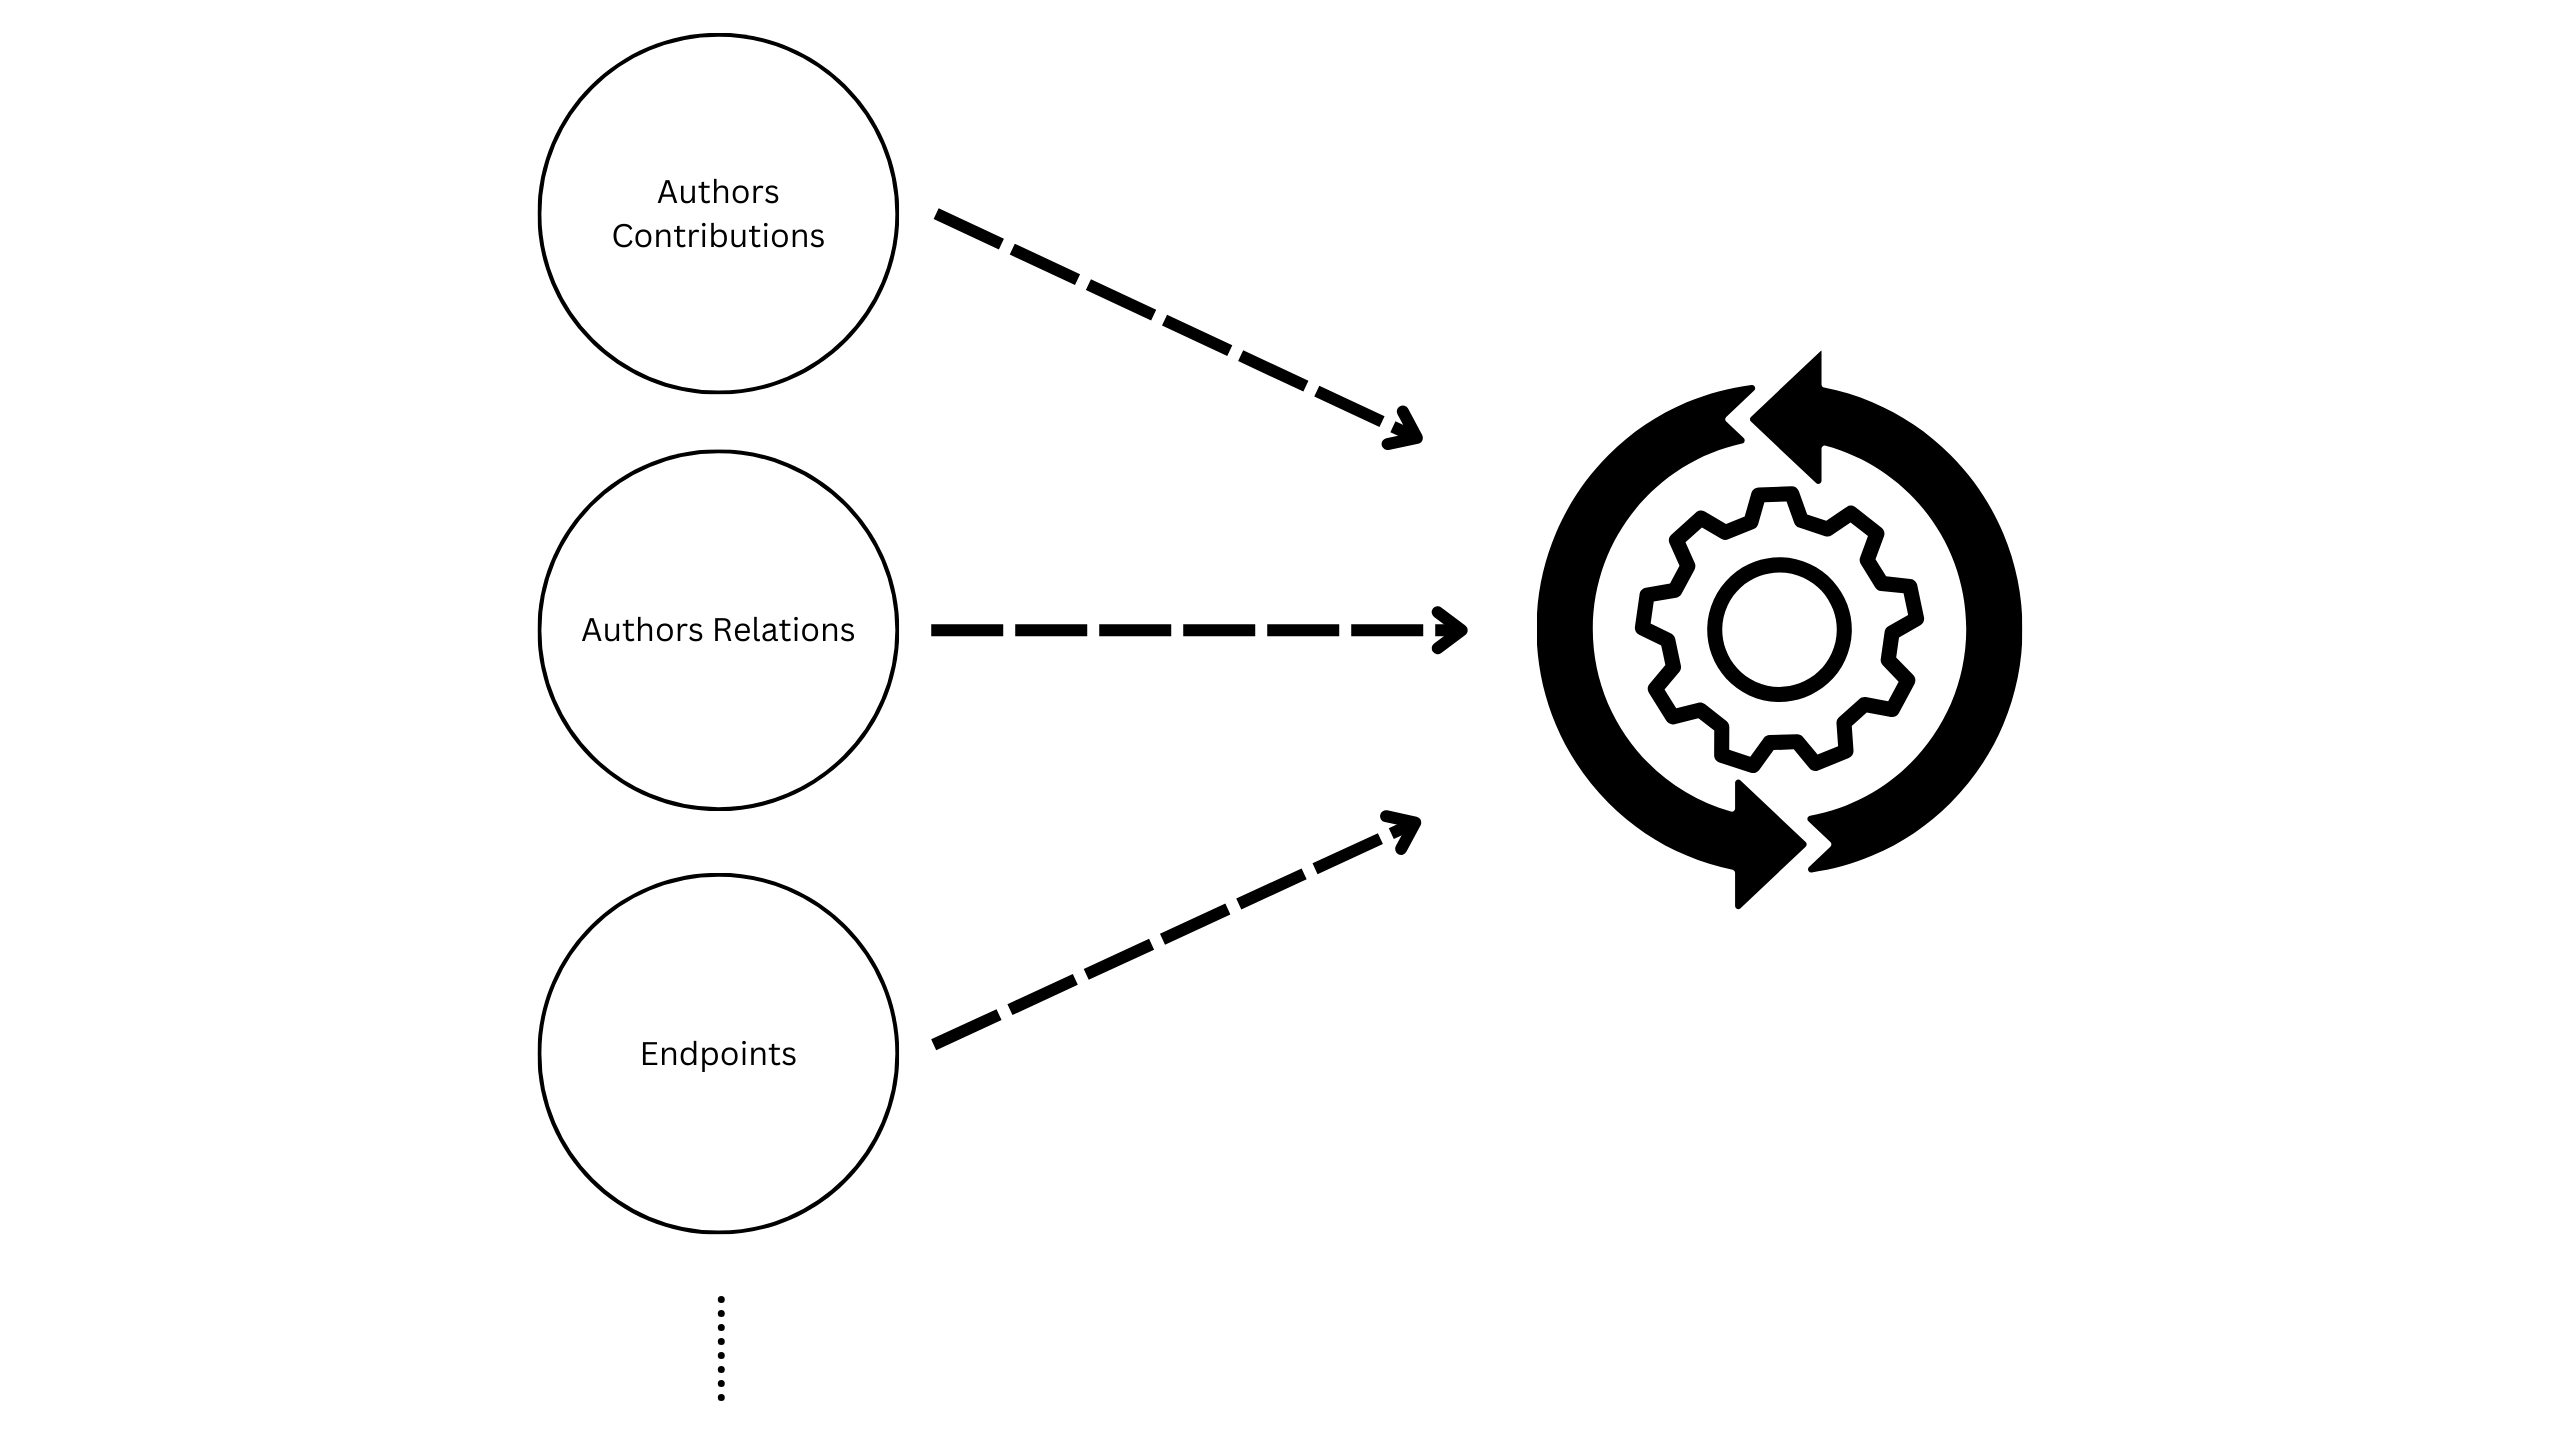
\includegraphics[width=1\textwidth]{figures/sst_working.png}
    \caption[Probes and SST]{Probes and SST}
    \label{fig_probes_sst}
\end{figure}

\subsubsection{Integration and Output}

The probes will extract the required data from the microservices and feed them to the SST for further processing. SST will generate output which will be used by the visualizer for further analysis and visualization.

\subsubsection{Data Management}

The output of the SST will be stored in a separate database to maintain and preserve historical records systematically. This approach ensures that the data is structured, organized, and easily retrievable from a centralized repository. By consolidating the data into a single repository, it not only simplifies access but also ensures a consistent format, which is critical for long-term usability and reliability. 

Storing the data in a database enhances its integrity by eliminating inconsistencies and reducing complexities, such as duplicate entries. This structure allows analysts or analysis tools to focus on extracting meaningful insights without the additional work of cleaning or reorganizing raw data.

Additionally, a dedicated database supports scalability, meaning it can accommodate larger datasets as the system evolves. It also offers improved data management capabilities, such as access controls and backup solutions, ensuring the data remains protected and readily available for future use.

\subsection{Visualizer}\label{subsec:component-visualizer}

If you need to use quotes, type it ``like this''.

\section{Referencing}
These are some sample references to GAMYGDALA~\citep{popescu2014gamygdala} from 
the \texttt{references.bib} file and state effects of 
cognition~\citep{hudlicka2002time} from the \texttt{references\_another.bib} 
file. These references are not in the same .bib file.

\section{Figures}
This is a single image figure (Figure~\ref{fig_singleenv}):

\begin{figure}[ht]
    \centering
    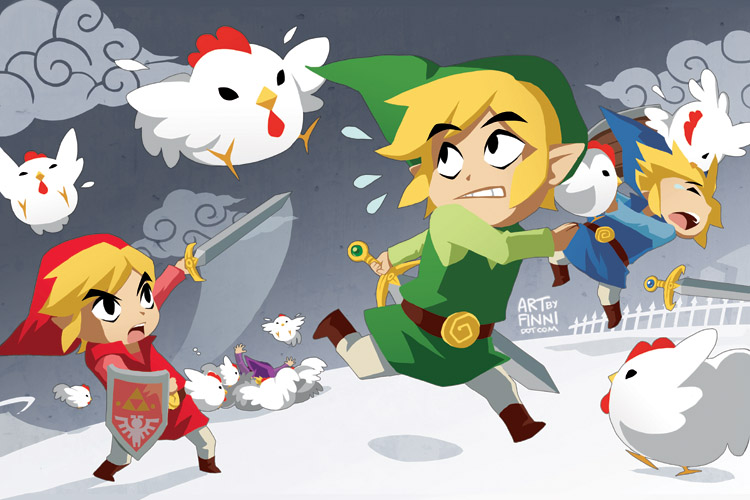
\includegraphics[width=0.6\textwidth]{figures/Sample/tumblr_static_eaceks0rfxsss8o4swscw40wo.jpg}
    \caption[Single Figure Environment Listed Title]{This is a single figure 
    environment}
    \label{fig_singleenv}
\end{figure}

This is a multi-image figure with a top (Figure~\ref{fig_multienv_1}) and bottom (Figure~\ref{fig_multienv_2}) aligned subfigures:

\begin{figure}[ht]
	\centering
	\begin{subfigure}[t]{\textwidth}
		\centering
		
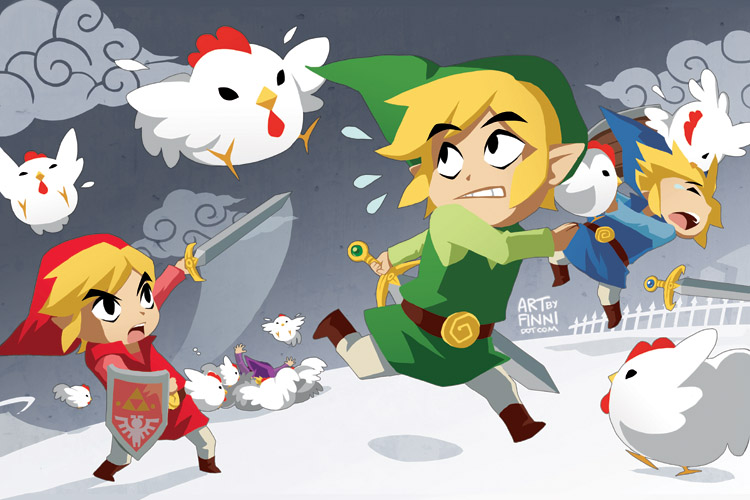
\includegraphics[width=0.7\textwidth]{figures/Sample/tumblr_static_eaceks0rfxsss8o4swscw40wo.jpg}
		\caption{Figure 1}
		\label{fig_multienv_1}
	\end{subfigure}
	~
	\begin{subfigure}[t]{\textwidth}
		\centering
		
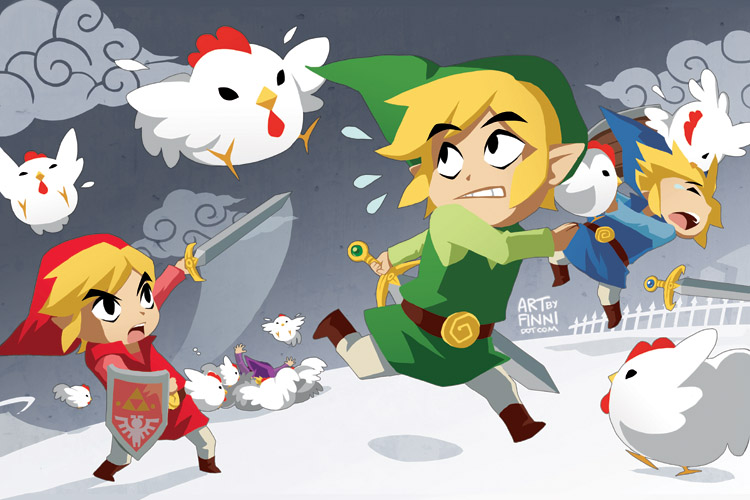
\includegraphics[width=0.7\textwidth]{figures/Sample/tumblr_static_eaceks0rfxsss8o4swscw40wo.jpg}
		\caption{Figure 2}
		\label{fig_multienv_2}
	\end{subfigure}
	
	\caption{A Multi-Figure Environment}
	\label{fig_multienv}
\end{figure}

\section{Tables}

Here is a sample table (Table~\ref{tab_sample}):

	\begin{table}[ht]
	\centering
	\begin{tabular}{ m{0.2\textwidth} m {0.1\textwidth} m{0.15\textwidth} }
		\toprule
		A & $\longleftrightarrow$ & B \\
		C & $\longleftrightarrow$ & D \\
		\bottomrule	
	\end{tabular}	
	\caption{A sample table}	
	\label{tab_sample}
\end{table}

\subsection{Long Tables}
A sample long table is shown in Appendix~\ref{appendix_b}.

\section{Equations}

Here is a sample equation (Equation~\ref{eq_lineslope}):

\begin{equation} \label{eq_lineslope}
	y = mx + b
\end{equation}                  
       \setcounter{figure}{0}
       \setcounter{equation}{0}
       \setcounter{table}{0}

  \chapter{Conclusion}

\section{Referencing}
These are some sample references to GAMYGDALA~\citep{popescu2014gamygdala} from 
the \texttt{references.bib} file and state effects of 
cognition~\citep{hudlicka2002time} from the \texttt{references\_another.bib} 
file. These references are not in the same .bib file.

\section{Figures}
This is a single image figure (Figure~\ref{fig_singleenv}):

\begin{figure}[ht]
    \centering
    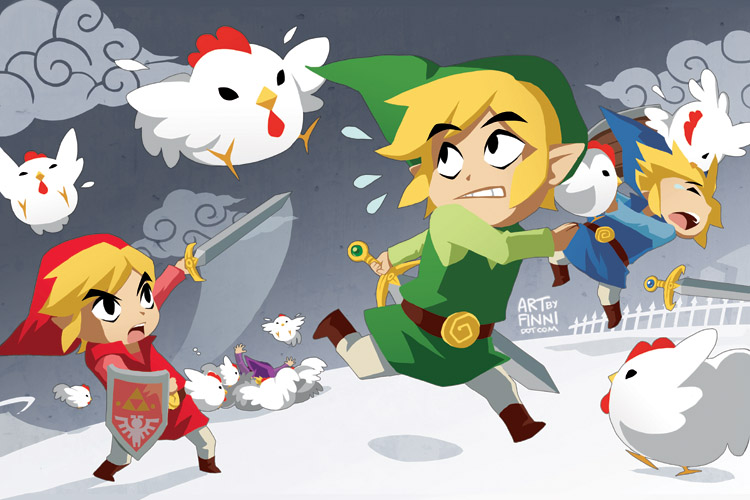
\includegraphics[width=0.6\textwidth]{figures/Sample/tumblr_static_eaceks0rfxsss8o4swscw40wo.jpg}
    \caption[Single Figure Environment Listed Title]{This is a single figure 
    environment}
    \label{fig_singleenv}
\end{figure}

This is a multi-image figure with a top (Figure~\ref{fig_multienv_1}) and bottom (Figure~\ref{fig_multienv_2}) aligned subfigures:

\begin{figure}[ht]
	\centering
	\begin{subfigure}[t]{\textwidth}
		\centering
		
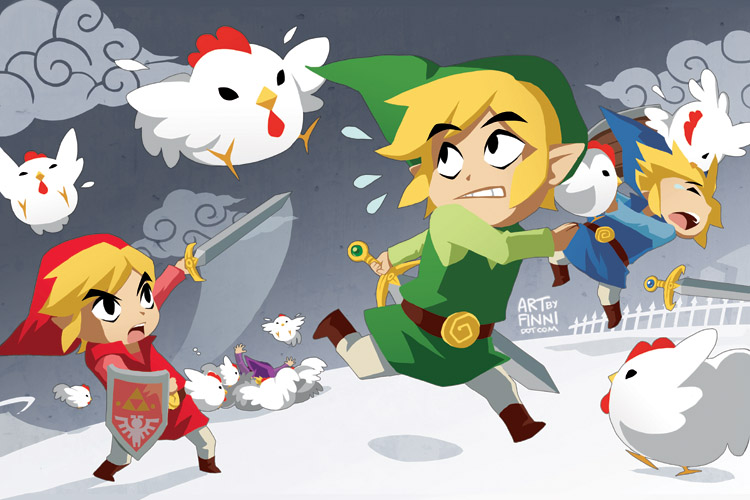
\includegraphics[width=0.7\textwidth]{figures/Sample/tumblr_static_eaceks0rfxsss8o4swscw40wo.jpg}
		\caption{Figure 1}
		\label{fig_multienv_1}
	\end{subfigure}
	~
	\begin{subfigure}[t]{\textwidth}
		\centering
		
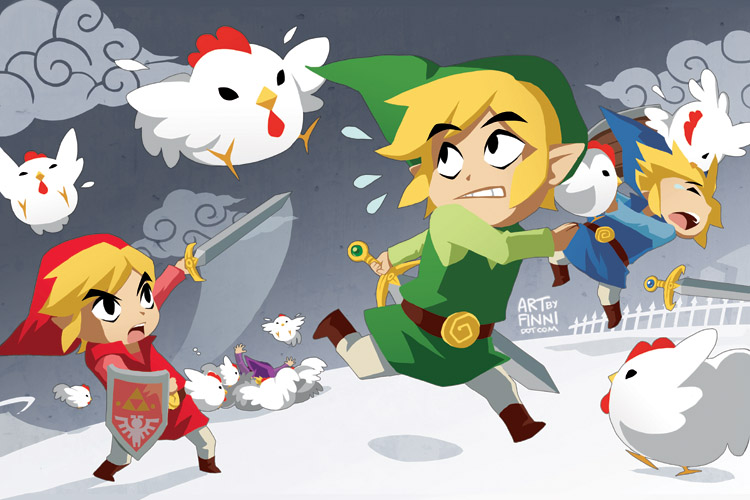
\includegraphics[width=0.7\textwidth]{figures/Sample/tumblr_static_eaceks0rfxsss8o4swscw40wo.jpg}
		\caption{Figure 2}
		\label{fig_multienv_2}
	\end{subfigure}
	
	\caption{A Multi-Figure Environment}
	\label{fig_multienv}
\end{figure}

\section{Tables}

Here is a sample table (Table~\ref{tab_sample}):

	\begin{table}[ht]
	\centering
	\begin{tabular}{ m{0.2\textwidth} m {0.1\textwidth} m{0.15\textwidth} }
		\toprule
		A & $\longleftrightarrow$ & B \\
		C & $\longleftrightarrow$ & D \\
		\bottomrule	
	\end{tabular}	
	\caption{A sample table}	
	\label{tab_sample}
\end{table}

\subsection{Long Tables}
A sample long table is shown in Appendix~\ref{appendix_b}.

\section{Equations}

Here is a sample equation (Equation~\ref{eq_lineslope}):

\begin{equation} \label{eq_lineslope}
	y = mx + b
\end{equation}
        \setcounter{figure}{0}
        \setcounter{equation}{0}
        \setcounter{table}{0}

\begin{appendix}
    \chapter{Your Appendix}
\label{appendix_a}

Your appendix goes here.

        \setcounter{figure}{0}
        \setcounter{equation}{0}
        \setcounter{table}{0}

    \chapter{Scenario Validation}\label{appendix_b}

\sloppy
The images related to scenario validations can be found from the project's Google Drive\footnote {\url{https://drive.google.com/drive/u/1/folders/1uTl1b0Fq_30UqRpwzeT3SyYyPLVKFt__}}. The following table includes the brief details of each image.

\begin{longtable}{|p{0.3\textwidth}|p{0.6\textwidth}|}
\hline
Image Name & Detail \\
\hline
\endfirsthead

\hline
Image Name & Detail \\
\hline
\endhead

\hline
\endfoot

\hline
\endlastfoot

% Data 1 & Data 2 \\

\end{longtable}


        \setcounter{figure}{0}
        \setcounter{equation}{0}
        \setcounter{table}{0}
\end{appendix}

% The bibliography is set up to allow for multiple bib files
\bibliographystyle{ACM-Reference-Format}
\bibliography{refs/references,refs/references_another,refs/articles,refs/inproceedings,refs/misc}

\label{NumDocumentPages}

\end{document}
% ********************************
